\documentclass[conference]{IEEEtran}

\usepackage{url}
\usepackage{graphicx}

% correct bad hyphenation here
\hyphenation{op-tical net-works semi-conduc-tor}

\begin{document}
% paper title
% can use linebreaks \\ within to get better formatting as desired
\title{Multirelational Association Mining with Ferda}

\author{\IEEEauthorblockN{Martin Ralbovsk\'{y} and Alexander Kuzmin}
\IEEEauthorblockA{Department of Information and Knowledge Engineering\\
University of Economics, Prague\\
W. Churchill Sq.~4, 130 67 Praha~3, Czech Republic\\
Email: martin.ralbovsky@gmail.com, alexander.kuzmin@gmail.com}}

% use for special paper notices
%\IEEEspecialpapernotice{(Invited Paper)}

% make the title area
\maketitle

\begin{abstract}
%\boldmath
The abstract goes here.
\end{abstract}
% IEEEtran.cls defaults to using nonbold math in the Abstract.
% This preserves the distinction between vectors and scalars. However,
% if the conference you are submitting to favors bold math in the abstract,
% then you can use LaTeX's standard command \boldmath at the very start
% of the abstract to achieve this. Many IEEE journals/conferences frown on
% math in the abstract anyway.

% no keywords

% For peer review papers, you can put extra information on the cover
% page as needed:
% \ifCLASSOPTIONpeerreview
% \begin{center} \bfseries EDICS Category: 3-BBND \end{center}
% \fi
%
% For peerreview papers, this IEEEtran command inserts a page break and
% creates the second title. It will be ignored for other modes.
\IEEEpeerreviewmaketitle

\section{Introduction}
\label{section:introduction}

Association rules mining is an important technique widely used in the
KDD community \cite{KDNuggets}. The classical algorithm for association rules 
mining, \emph{apriori} \cite{Agrawal2} is restricted to mining over a single 
relation composed of a set of binary attributes. 

There are some approaches that extend the classical algorithm with ability
of mining over multiple relations. Dehaspe and De Raedt\cite{Warmr} use 
techniques from the field of inductive logical programming used in their 
\emph{WARMR} algorithm. It is suitable for complex structure of relations 
and had several successful applications. Other approach \cite{Connection}
adapts \emph{support} and \emph{confidence} measures and calculates them on
tables without joining them. These approaches are based on the \emph{apriori}
algorithm.

There are also approaches to extend expressing power of association rules.
By far the most significant work in this field is the ongoing research of
the GUHA method \cite{GUHA1, GUHA2}. GUHA is the an original method of 
exploratory data analysis that is nowadays researched mainly in context of
generalizing association rules \cite{Rauch2, Alternative}. Attemts to
use generalized association rules also for multirelational data were made
\cite{Rauch1, Karban}. The technique uses star schema of the 
database\footnote{One master table and several detail tables.} and introduced
\emph{virtual attribute}, attribute that is computed from the detail tables
and acts as attribute of master table. There are two types of 
\emph{virtual attributes} presented: SQL transformation or generalized
association rule mined above the detail table\footnote{To be explained
later}. The latter cannot be obtained by any of the methods based on 
\emph{apriori} algorithm. 

Although the theory for multirelational extentions of the GUHA association
mining is well developed, until now there was a lack of successful 
implementation. In our Ferda environment, we implemented the multirelational
extentions of GUHA generalized association rules and conducted some very
useful experiments to show advisability of these rules. The aim of this paper
is to present multirelational association rules based on \emph{virtual attributes}
and to demonstrate their implementation in the Ferda system. 

Paper is structured as follows: Section \ref{section:principles} explains in brief
the principles of multirelational association mining with \emph{virtual attributes}.
Section \ref{section:ferda} describes the demonstrated system. Section 
\ref{section:features} states the features of the system to be demonstrated
and section \ref{section:conclusion} concludes the paper. 

\section{Principles of Multirelational Association mining}
\label{section:principles}

\subsection{Generalized Association Rules}
\label{section:generalized}
Let us first explain the generalized association rules in sense of GUHA method
\cite{Rauch1,Rauch2,Alternative}\footnote{For simplicity, we focus only on 
\emph{unconditional rules}. More on \emph{conditional rules} can be found in 
\cite{Rauch2}.}. Generalized association rules mined by procedure 4FT \cite{Alternative}
extend the ``classical'' association rules from \emph{apriori} procedure
X$\rightarrow$Y, where X and Y are sets of items, in two ways. 

The first way is to
enable \emph{Boolean attributes} for antecedent and consequent. \emph{Boolean attributes}
are recursive structures that enable conjunctions, disjunctions and negations of
combinations of individual items. Details can be found in \cite{Ralbovsky}.

The second way is to enable expressing more general kind of dependency between 
antecedent and consequent then \emph{confidence} and \emph{support}. We call these 
dependencies \emph{4ft-quantifiers}. The generalized association rule can be written
in form \mbox{$\varphi \approx \psi$}, where $\varphi$ and $\psi$ are 
\emph{Boolean attributes} and $\approx$ is a \emph{4ft-quantifier}.
The quantifier is computed on the basis of \emph{4ft-table}, as shown in 
Table \ref{table:4FTcontingency}.

\begin{table}[ht]
	\begin{center}
		\begin{tabular}{r|c|c}
		{\b M}        & $ \psi $ &  $ \neg \psi $ \\
		\hline
		     $  \varphi $  &  \ \ $ a  \ \ $    & $  \ \ b \ \  $    \\
		\hline
		   $ \neg \varphi $  &  $ c $    & $ d $    \\
		\end {tabular}
	\end{center}
	\caption{4FT contingency table}
	\label{table:4FTcontingency}
\end{table}

A \emph{4ft table} is a quadruple of natural numbers 
\emph{$\langle$a, b, c, d$\rangle$}
so that: $a$ is the number of object from the data matrix satisfying $\varphi$ and 
$\psi$ (likewise for other numbers). 

The \emph{above average dependence} quantifier is example of such. It is defined 
by the following condition:
$$\frac{a}{a+b}\geq(1+p)\frac{a+c}{a+b+c+d} \wedge a \leq Base$$
where $p$ and $Base$ are user-defined parameters. It can be verbally interpreted
as \emph{Among object satisfying $\varphi$, there are at least 100p per cent 
more objects satisfying $\psi$ then among all observed objects and there are
at least Base observed objects satisfying $\varphi$ and $\psi$.}

\subsection{Virtual attributes}
\label{section:attributes}

We explain our method on following example: there are two tables concerning clients
of a bank. The master table contains information about clients' accounts and the detail 
table contains information about transactions of individual clients\footnote{The
example was greatly inspired by data describing clients of virtual bank Barbora. The
dataset was examined e.g. during the PKDD 1999 Discovery challenge, see 
\url{http://lisp.vse.cz/challenge}.}.

\emph{Virtual attributes} are attributes from detail data tables, that are created
during the process of association rules verification and are treated as normal attributes
of master table although not physically stored. The Ferda system allows creation of
two types of \emph{virtual attributes}: \emph{aggregation attributes} and \emph{hypotheses
attributes}. 

\emph{Aggregation attributes} can be created as SQL aggregations over
a detail table. Attribute stating the average amount of money transfered by a client
is an example of \emph{aggregation attribute}. We will not focus on \emph{aggregation
attributes}, because they can be also imported into the master data table by corresponding
SQL transformations.

\emph{Hypotheses attributes} are of more interest. They represent a generalized
association rule (as explained above), which is true or false for each key item
of the master table. Example of such attribute can be \emph{client that often
pays by credit card}, which can be formally written as 
$$ClientID \approx Payment(CreditCard)$$
with a suitable \emph{4ft-quantifier} $\approx$. It is obvious, that this rule
may be very useful to use in the master table concerning clients' accounts. We
name the \emph{virtual attribute} $ClientPayingByCreditCard$. Then one can 
examine status of a client based on client's payments and address. Example of
such generalized association rule is
$$District(SouthEast) \& ClientPayingByCreditCard$$
$$\approx Status(good)$$
Note that these types of rules cannot be obtained by any other method mentioned in
section \ref{section:introduction}.

Issues concerning \emph{hypotheses attributes} by far exceed the scope of this paper.
As well as WARMR, construction of \emph{hypotheses attributes} suffer from explosion
of hypotheses space. \cite{Karban} gives more information about this problem. 
Interpretation of \emph{hypotheses attributes} poses another issue. Vast
majority of association rules created from the detail data table are not interpretable
within the master data table. Yet there are some constrains according to which
interpretable rules can be created. The matter is at present under research. 

\section{The Ferda DataMiner}
\label{section:ferda}
Ferda DataMiner\footnote{\url{http://sourceforge.net/projects/ferda}} (or Ferda)
is the newest system implementing the GUHA method\cite{GUHA1, GUHA2}.
It envolved from the older \emph{LISp--Miner} 
system\footnote{\url{http://lispminer.vse.cz}}. 

Apart from implementing 4FT, procedure for mining generalized association
rules (as described in section \ref{section:generalized}) and its multirelational 
version, Ferda implements five other relational and one multirelational 
procedures for finding interesting patterns in the data, based on the GUHA 
method. 

One of main features of the Ferda system is visualization of the data mining task
setup. Figure \ref{fig:environment} shows the working environment. User constructs
the task by connecting and setting visual elements called \emph{boxes}. Unlike in
other system, \emph{box} does not represent part of the mining process. It represents
a function, that has input parameters and computes its output. At present, language
of boxes' functions is not recursive, however we are working on a fully recursive
language with standard functional constructs like arrays and $\lambda$ function. 

\begin{figure}[!t]
\centering
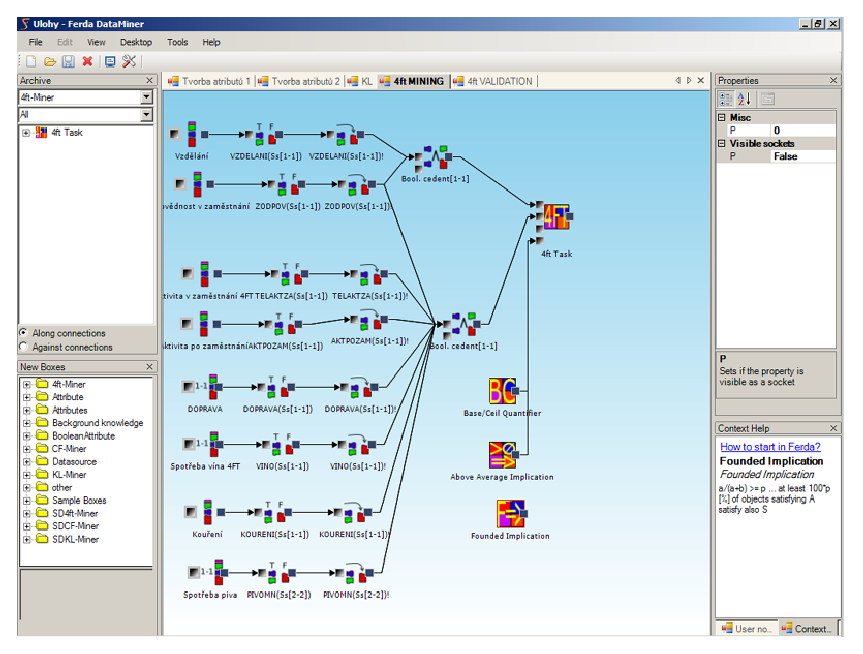
\includegraphics[width=3in]{ferda.eps}
% where an .eps filename suffix will be assumed under latex, 
% and a .pdf suffix will be assumed for pdflatex; or what has been declared
% via \DeclareGraphicsExtensions.
\caption{The Ferda environment}
\label{fig:environment}
\end{figure}

Ferda has also some implementation features worth mentioning. The program is written
under GPL license and runs on .NET Framework and Mono. Ferda is a highly modular 
environment, each \emph{box} can run on different computer over the network and can
be written in one of several programming languages. This is achieved by using the Ice
middleware\footnote{\url{http://www.zeroc.com}}. More details on \emph{boxes} 
and implementation of Ferda can be found in \cite{Ferda}.

\section{Demonstrated features}
\label{section:features}

We would like to present the Ferda system, focusing on usage of multirelational 
association mining, mainly \emph{hypotheses attributes}. After short introduction 
of the Ferda environment, we will present various multirelational association
mining tasks. Figure \ref{fig:example} shows one of such. 

\begin{figure}[!t]
\centering
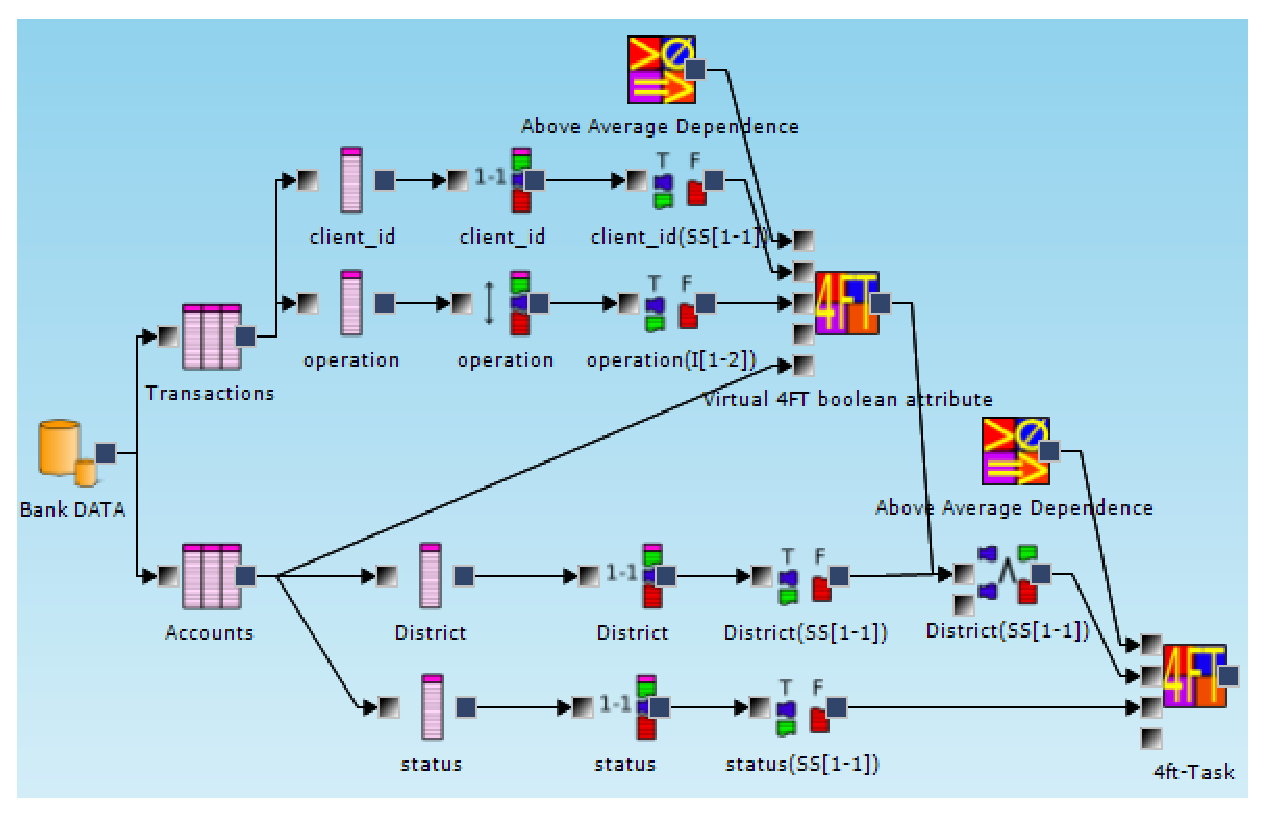
\includegraphics[width=3.2in]{Example.eps}
% where an .eps filename suffix will be assumed under latex, 
% and a .pdf suffix will be assumed for pdflatex; or what has been declared
% via \DeclareGraphicsExtensions.
\caption{Example of multirelational task setting}
\label{fig:example}
\end{figure}

The \emph{hypotheses attribute} task setting is located in the upper part of the 
figure. The setting corresponds to example of \emph{hypotheses attribute} from section 
\ref{section:attributes}. It examines relations between clients and types of operations (deposit, withdrawal or credit card payment). \emph{Above average dependence} quantifier
is used. 

Lower part of figure \ref{fig:example} shows task setting of the master table. Information
about client's district in conjunction with \emph{hypotheses attribute} are examined 
against status of the client. The setting again corresponds to exemplary association 
rule from section \ref{section:attributes}. Note similar appearance of the master 
table task \emph{box} and also the \emph{hypotheses attribute box} -- they represent 
modifications of the 4FT procedure. Also note how inputs of the master table task 
box represents setting of generalized association rules, \mbox{$\varphi \approx \psi$}.
$$$$
We would also like to present, how \emph{hypotheses attribute} setting can affect
the hypotheses space and thus the running times. So far, our experiments have been
based on examining the Barbora dataset. This dataset contains only generated data, 
so observed rules are not relevant in the real world. We will try to find another
source of data and mine interesting multirelational rules. After the implementation,
we also encountered problems with interpreting multirelational rules and with 
setting of intepretable tasks. The issue is a matter of research and by the time 
of the conference, we should bring findings. 

\section{Conclusion}
\label{section:conclusion}
The conclusion goes here.

\section*{Acknowledgment}

This work was supported by the project MSM6138439910 of the
Ministry of Education of the Czech Republic, project IG407056 of University
of Economics, Prague and by the project 201/05/0325 of the Czech Science
Foundation. 

We would like to thanks our research colleagues Jan Rauch,
Tom\'{a}\v{s} Kucha\v{r} and Michal Kov\'{a}\v{c} for help, valuable comments 
and reviews.

% trigger a \newpage just before the given reference
% number - used to balance the columns on the last page
% adjust value as needed - may need to be readjusted if
% the document is modified later
%\IEEEtriggeratref{8}
% The "triggered" command can be changed if desired:
%\IEEEtriggercmd{\enlargethispage{-5in}}

\begin{thebibliography}{1}

\bibitem{Agrawal2}
Agrawal R., Mannila H., Srikant R., Toivonen H., Verkamo A.:
\emph{Fast discovery of association rules}. Fayyad, U., Piatetsky-Shapiro, G., Smyth, 
P., Uthurusamy, R., eds.: Advances in Knowledge Discovery and Data Mining. AAAI Press, 
Menlo Park (1996) p.~307~--~328

\bibitem{Warmr}
Dehaspe L., De Raedt L.:
\emph{Mining Association Rules in Multiple Relations}. In Proceedings of the 7th
International Workshop on Inductive Logical Programming, Volume 1297, LNAI,
pp. 125--132, Springer-Verlag, 1997

\bibitem{Ferda}
Kov\'{a}\v{c} M., Kucha\v{r} T., Kuzmin A., Ralbovsk\'{y} M.: \emph{Ferda, 
New Visual Environment for Data Mining}. Znalosti 2006, 
Conference on Data Mining, Hradec Kr\'{a}lov\'{e} 2006, p.~118~--~129 (in Czech)

\bibitem{GUHA1}
H\'{a}jek P., Havel I., Chytil M.: \emph{The GUHA method of
automatic hypotheses determination}. Computing 1, 1966, p.~293~--~308

\bibitem{GUHA2}
H\'{a}jek P., Havr\'{a}nek, T.: \emph{Mechanising Hypothesis
Formation - Mathematical  Foundations  for  a   General  Theory}.
Springer-Verlag: Berlin  - Heidelberg - New York, 1978.

\bibitem{Karban}
Karban T.: \emph{Relational Data Mining and GUHA}. in Richta K., 
Sn\'{a}\v{s}el V., Pokorn\'{y} J.(eds.): Proceedings of the 5th annual
workshop DATESO 2005(Databases, Texts, Specifications and Objects),
ISBN:80-01-03204-3, pp.103--112

\bibitem{KDNuggets}
KDNuggets Polls, \emph{Data mining/analytic techniques you use frequently}.
\url{www.kdnuggets.com/polls/2005/data_mining_techniques.htm}

\bibitem{Connection}
Pizzi, L.C., Ribeiro, M.X., Vieira, M.T.P.:
\emph{Analysis of Hepatitis Dataset using Multirelational Association Rules}. 
ECML/PKDD Discovery Challenge, 2005.

\bibitem{Rauch1}
Rauch J.: \emph{Interesting Association Rules and Multi-relational Association
Rules}. Communications of Institute of Information and Computing Machinery, Taiwan.
Vol. 5, No 2, May 2002. pp. 77--82

\bibitem{Rauch2}
Rauch J.: \emph{Logic of Association Rules}. In: Applied Inteligence, Vol. 22,
Issue 1, p.~9~--~28

\bibitem{Alternative}
Rauch J., \v{S}im\accent23unek, M.: \emph{An Alternative Approach to Mining
Association Rules} Lin T Y, Ohsuga S, Liau C J, and Tsumoto S (eds):
Foundations of Data Mining and Knowledge Discovery, Springer-Verlag, 2005
p.~219~--~239

\bibitem{Ralbovsky}
Ralbovsk\'{y} M., Kucha\v{r} T.: 
\emph{Using Disjunctions in Association Mining}. 
In: Perner P.: Advances in Data Mining, Springer-Verlag 2007, to appear

\end{thebibliography}

% that's all folks
\end{document}


%\hfill January 11, 2007

% An example of a floating figure using the graphicx package.
% Note that \label must occur AFTER (or within) \caption.
% For figures, \caption should occur after the \includegraphics.
% Note that IEEEtran v1.7 and later has special internal code that
% is designed to preserve the operation of \label within \caption
% even when the captionsoff option is in effect. However, because
% of issues like this, it may be the safest practice to put all your
% \label just after \caption rather than within \caption{}.
%
% Reminder: the "draftcls" or "draftclsnofoot", not "draft", class
% option should be used if it is desired that the figures are to be
% displayed while in draft mode.
%
%\begin{figure}[!t]
%\centering
%\includegraphics[width=2.5in]{myfigure}
% where an .eps filename suffix will be assumed under latex, 
% and a .pdf suffix will be assumed for pdflatex; or what has been declared
% via \DeclareGraphicsExtensions.
%\caption{Simulation Results}
%\label{fig_sim}
%\end{figure}

% Note that IEEE typically puts floats only at the top, even when this
% results in a large percentage of a column being occupied by floats.


% An example of a double column floating figure using two subfigures.
% (The subfig.sty package must be loaded for this to work.)
% The subfigure \label commands are set within each subfloat command, the
% \label for the overall figure must come after \caption.
% \hfil must be used as a separator to get equal spacing.
% The subfigure.sty package works much the same way, except \subfigure is
% used instead of \subfloat.
%
%\begin{figure*}[!t]
%\centerline{\subfloat[Case I]\includegraphics[width=2.5in]{subfigcase1}%
%\label{fig_first_case}}
%\hfil
%\subfloat[Case II]{\includegraphics[width=2.5in]{subfigcase2}%
%\label{fig_second_case}}}
%\caption{Simulation results}
%\label{fig_sim}
%\end{figure*}
%
% Note that often IEEE papers with subfigures do not employ subfigure
% captions (using the optional argument to \subfloat), but instead will
% reference/describe all of them (a), (b), etc., within the main caption.


% An example of a floating table. Note that, for IEEE style tables, the 
% \caption command should come BEFORE the table. Table text will default to
% \footnotesize as IEEE normally uses this smaller font for tables.
% The \label must come after \caption as always.
%
%\begin{table}[!t]
%% increase table row spacing, adjust to taste
%\renewcommand{\arraystretch}{1.3}
% if using array.sty, it might be a good idea to tweak the value of
% \extrarowheight as needed to properly center the text within the cells
%\caption{An Example of a Table}
%\label{table_example}
%\centering
%% Some packages, such as MDW tools, offer better commands for making tables
%% than the plain LaTeX2e tabular which is used here.
%\begin{tabular}{|c||c|}
%\hline
%One & Two\\
%\hline
%Three & Four\\
%\hline
%\end{tabular}
%\end{table}


% Note that IEEE does not put floats in the very first column - or typically
% anywhere on the first page for that matter. Also, in-text middle ("here")
% positioning is not used. Most IEEE journals/conferences use top floats
% exclusively. Note that, LaTeX2e, unlike IEEE journals/conferences, places
% footnotes above bottom floats. This can be corrected via the \fnbelowfloat
% command of the stfloats package.
